%chapter 12

\chapter{Tuplas}

Este capítulo presenta otro tipo incorporado, la tupla, y luego muestra cómo las listas, los diccionarios y las tuplas trabajan juntos. También se presenta una característica útil para listas de argumentos de longitud variable: los operadores de reunión y dispersión.

Una nota: no hay consenso sobre cómo pronunciar "tuple". Algunas personas dicen "tú-pl", que rima con "sú-pl". Pero en el contexto de programación, la mayoría dice "tu-ple", que rima con "cuádruple".

\section{Las tuplas son inmutables}

Una tupla es una secuencia de valores. Los valores pueden ser de cualquier tipo y están indexados por enteros, por lo que en ese aspecto las tuplas son muy similares a las listas. La diferencia importante es que las tuplas son inmutables.

Sintácticamente, una tupla es una lista de valores separados por comas:

\begin{lstlisting}[language=Python]
>>> t = 'a', 'b', 'c', 'd', 'e'
\end{lstlisting}

Aunque no es necesario, es común encerrar las tuplas entre paréntesis:

\begin{lstlisting}[language=Python]
>>> t = ('a', 'b', 'c', 'd', 'e')
\end{lstlisting}

Para crear una tupla con un solo elemento, debes incluir una coma final:

\begin{lstlisting}[language=Python]
>>> t1 = 'a',
>>> type(t1)
<class 'tuple'>
\end{lstlisting}

Un valor entre paréntesis no es una tupla:

\begin{lstlisting}[language=Python]
>>> t2 = ('a')
>>> type(t2)
<class 'str'>
\end{lstlisting}

Otra forma de crear una tupla es usando la función incorporada \texttt{tuple}. Sin argumentos, crea una tupla vacía:

\begin{lstlisting}[language=Python]
>>> t = tuple()
>>> t
()
\end{lstlisting}

Si el argumento es una secuencia (cadena, lista o tupla), el resultado es una tupla con los elementos de la secuencia:

\begin{lstlisting}[language=Python]
>>> t = tuple('lupins')
>>> t
('l', 'u', 'p', 'i', 'n', 's')
\end{lstlisting}

Como \texttt{tuple} es el nombre de una función incorporada, debes evitar usarlo como nombre de variable.

La mayoría de los operadores de listas también funcionan con tuplas. El operador corchete indexa un elemento:

\begin{lstlisting}[language=Python]
>>> t = ('a', 'b', 'c', 'd', 'e')
>>> t[0]
'a'
\end{lstlisting}

Y el operador de segmento selecciona un rango de elementos:

\begin{lstlisting}[language=Python]
>>> t[1:3]
('b', 'c')
\end{lstlisting}

Pero si intentas modificar uno de los elementos de la tupla, obtendrás un error:

\begin{lstlisting}[language=Python]
>>> t[0] = 'A'
TypeError: object doesn't support item assignment
\end{lstlisting}

Como las tuplas son inmutables, no puedes modificar sus elementos. Pero puedes reemplazar una tupla por otra:

\begin{lstlisting}[language=Python]
>>> t = ('A',) + t[1:]
>>> t
('A', 'b', 'c', 'd', 'e')
\end{lstlisting}

Los operadores relacionales funcionan con tuplas y otras secuencias; Python comienza comparando el primer elemento de cada secuencia. Si son iguales, pasa a los siguientes elementos, y así sucesivamente, hasta encontrar elementos que difieran. Los elementos posteriores no se consideran (incluso si son muy grandes):

\begin{lstlisting}[language=Python]
>>> (0, 1, 2) < (0, 3, 4)
True
>>> (0, 1, 2000000) < (0, 3, 4)
True
\end{lstlisting}

\section{Asignación de tuplas}

A menudo es útil intercambiar los valores de dos variables. Con asignaciones convencionales, debes usar una variable temporal. Por ejemplo, para intercambiar \texttt{a} y \texttt{b}:

\begin{lstlisting}[language=Python]
>>> temp = a
>>> a = b
>>> b = temp
\end{lstlisting}

Esta solución es engorrosa; la asignación de tuplas es más elegante:

\begin{lstlisting}[language=Python]
>>> a, b = b, a
\end{lstlisting}

El lado izquierdo es una tupla de variables; el lado derecho es una tupla de expresiones. Cada valor se asigna a su respectiva variable. Todas las expresiones del lado derecho se evalúan antes de cualquier asignación.

El número de variables a la izquierda y el número de valores a la derecha deben ser iguales:

\begin{lstlisting}[language=Python]
>>> a, b = 1, 2, 3
ValueError: too many values to unpack
\end{lstlisting}

En general, el lado derecho puede ser cualquier tipo de secuencia (cadena, lista o tupla). Por ejemplo, para dividir una dirección de correo electrónico en un nombre de usuario y un dominio, podrías escribir:

\begin{lstlisting}[language=Python]
>>> addr = 'monty@python.org'
>>> uname, domain = addr.split('@')
\end{lstlisting}

El valor de retorno de \texttt{split} es una lista con dos elementos; el primer elemento se asigna a \texttt{uname}, el segundo a \texttt{domain}:

\begin{lstlisting}[language=Python]
>>> uname
'monty'
>>> domain
'python.org'
\end{lstlisting}

\section{Tuplas como valores de retorno}

Estrictamente hablando, una función solo puede devolver un valor, pero si el valor es una tupla, el efecto es el mismo que devolver múltiples valores. Por ejemplo, si quieres dividir dos enteros y calcular el cociente y el resto, es ineficiente calcular \texttt{x//y} y luego \texttt{x\%y}. Es mejor calcular ambos al mismo tiempo.

La función incorporada \texttt{divmod} toma dos argumentos y devuelve una tupla de dos valores, el cociente y el resto. Puedes almacenar el resultado como una tupla:

\begin{lstlisting}[language=Python]
>>> t = divmod(7, 3)
>>> t
(2, 1)
\end{lstlisting}

O usar asignación de tuplas para almacenar los elementos por separado:

\begin{lstlisting}[language=Python]
>>> quot, rem = divmod(7, 3)
>>> quot
2
>>> rem
1
\end{lstlisting}

Aquí hay un ejemplo de una función que devuelve una tupla:

\begin{lstlisting}[language=Python]
def min_max(t):
    return min(t), max(t)
\end{lstlisting}

\texttt{max} y \texttt{min} son funciones incorporadas que encuentran los elementos más grandes y más pequeños de una secuencia. \texttt{min\_max} calcula ambos y devuelve una tupla de dos valores.

\section{Tuplas de argumentos de longitud variable}

Las funciones pueden tomar un número variable de argumentos. Un nombre de parámetro que comienza con \texttt{*} recoge los argumentos en una tupla. Por ejemplo, \texttt{printall} toma cualquier número de argumentos y los imprime:

\begin{lstlisting}[language=Python]
def printall(*args):
    print(args)
\end{lstlisting}

El parámetro de recolección puede tener cualquier nombre, pero \texttt{args} es convencional. Así funciona la función:

\begin{lstlisting}[language=Python]
>>> printall(1, 2.0, '3')
(1, 2.0, '3')
\end{lstlisting}

El complemento de recolección es dispersión. Si tienes una secuencia de valores y quieres pasarla a una función como múltiples argumentos, puedes usar el operador \texttt{*}. Por ejemplo, \texttt{divmod} toma exactamente dos argumentos; no funciona con una tupla:

\begin{lstlisting}[language=Python]
>>> t = (7, 3)
>>> divmod(t)
TypeError: divmod expected 2 arguments, got 1
\end{lstlisting}

Pero si dispersas la tupla, funciona:

\begin{lstlisting}[language=Python]
>>> divmod(*t)
(2, 1)
\end{lstlisting}

Muchas funciones incorporadas usan tuplas de argumentos de longitud variable. Por ejemplo, \texttt{max} y \texttt{min} pueden tomar cualquier número de argumentos:

\begin{lstlisting}[language=Python]
>>> max(1, 2, 3)
3
\end{lstlisting}

Pero \texttt{sum} no:

\begin{lstlisting}[language=Python]
>>> sum(1, 2, 3)
TypeError: sum expected at most 2 arguments, got 3
\end{lstlisting}

Como ejercicio, escribe una función llamada \texttt{sum\_all} que tome cualquier número de argumentos y devuelva su suma.

\section{Listas y tuplas}

\texttt{zip} es una función incorporada que toma dos o más secuencias y las entrelaza. El nombre de la función se refiere a una cremallera, que entrelaza dos filas de dientes.

Este ejemplo entrelaza una cadena y una lista:

\begin{lstlisting}[language=Python]
>>> s = 'abc'
>>> t = [0, 1, 2]
>>> zip(s, t)
<zip object at 0x7f7d0a9e7c48>
\end{lstlisting}

El resultado es un objeto \texttt{zip} que sabe cómo iterar a través de los pares. El uso más común de \texttt{zip} es en un bucle \texttt{for}:

\begin{lstlisting}[language=Python]
>>> for pair in zip(s, t):
...     print(pair)
...
('a', 0)
('b', 1)
('c', 2)
\end{lstlisting}

Un objeto \texttt{zip} es un tipo de iterador, que es cualquier objeto que itera a través de una secuencia. Los iteradores son similares a las listas en algunos aspectos, pero a diferencia de las listas, no puedes usar un índice para seleccionar un elemento de un iterador.

Si quieres usar operadores y métodos de listas, puedes usar un objeto \texttt{zip} para crear una lista:

\begin{lstlisting}[language=Python]
>>> list(zip(s, t))
[('a', 0), ('b', 1), ('c', 2)]
\end{lstlisting}

El resultado es una lista de tuplas; en este ejemplo, cada tupla contiene un carácter de la cadena y el elemento correspondiente de la lista.

Si las secuencias no tienen la misma longitud, el resultado tiene la longitud de la más corta:

\begin{lstlisting}[language=Python]
>>> list(zip('Anne', 'Elk'))
[('A', 'E'), ('n', 'l'), ('n', 'k')]
\end{lstlisting}

Puedes usar asignación de tuplas en un bucle \texttt{for} para recorrer una lista de tuplas:

\begin{lstlisting}[language=Python]
t = [('a', 0), ('b', 1), ('c', 2)]
for letter, number in t:
    print(number, letter)
\end{lstlisting}

Cada vez que se recorre el bucle, Python selecciona la siguiente tupla en la lista y asigna los elementos a \texttt{letter} y \texttt{number}. La salida de este bucle es:

\begin{lstlisting}[language=Python]
0 a
1 b
2 c
\end{lstlisting}

Si combinas \texttt{zip}, \texttt{for} y asignación de tuplas, obtienes un patrón útil para recorrer dos (o más) secuencias al mismo tiempo. Por ejemplo, \texttt{has\_match} toma dos secuencias, \texttt{t1} y \texttt{t2}, y devuelve \texttt{True} si hay un índice \texttt{i} tal que \texttt{t1[i] == t2[i]}:

\begin{lstlisting}[language=Python]
def has_match(t1, t2):
    for x, y in zip(t1, t2):
        if x == y:
            return True
    return False
\end{lstlisting}

Si necesitas recorrer los elementos de una secuencia y sus índices, puedes usar la función incorporada \texttt{enumerate}:

\begin{lstlisting}[language=Python]
for index, element in enumerate('abc'):
    print(index, element)
\end{lstlisting}

El resultado de \texttt{enumerate} es un objeto \texttt{enumerate}, que itera una secuencia de pares; cada par contiene un índice (comenzando desde 0) y un elemento de la secuencia dada. En este ejemplo, la salida es:

\begin{lstlisting}[language=Python]
0 a
1 b
2 c
\end{lstlisting}

\section{Diccionarios y tuplas}

Los diccionarios tienen un método llamado \texttt{items} que devuelve una secuencia de tuplas, donde cada tupla es un par clave-valor.

\begin{lstlisting}[language=Python]
>>> d = {'a':0, 'b':1, 'c':2}
>>> t = d.items()
>>> t
dict_items([('c', 2), ('a', 0), ('b', 1)])
\end{lstlisting}

El resultado es un objeto \texttt{dict\_items}, que es un iterador que recorre los pares clave-valor. Puedes usarlo en un bucle \texttt{for} así:

\begin{lstlisting}[language=Python]
>>> for key, value in d.items():
...     print(key, value)
...
c 2
a 0
b 1
\end{lstlisting}

Como es de esperar en un diccionario, los elementos no tienen un orden particular.

En la otra dirección, puedes usar una lista de tuplas para inicializar un nuevo diccionario:

\begin{lstlisting}[language=Python]
>>> t = [('a', 0), ('c', 2), ('b', 1)]
>>> d = dict(t)
>>> d
{'a': 0, 'c': 2, 'b': 1}
\end{lstlisting}

Combinar \texttt{dict} con \texttt{zip} proporciona una forma concisa de crear un diccionario:

\begin{lstlisting}[language=Python]
>>> d = dict(zip('abc', range(3)))
>>> d
{'a': 0, 'c': 2, 'b': 1}
\end{lstlisting}

El método \texttt{update} de los diccionarios también toma una lista de tuplas y las agrega, como pares clave-valor, a un diccionario existente.

Es común usar tuplas como claves en diccionarios (principalmente porque no puedes usar listas). Por ejemplo, un directorio telefónico podría mapear pares apellido, nombre a números de teléfono. Suponiendo que hemos definido \texttt{last}, \texttt{first} y \texttt{number}, podríamos escribir:

\begin{lstlisting}[language=Python]
directory[last, first] = number
\end{lstlisting}

La expresión entre corchetes es una tupla. Podríamos usar asignación de tuplas para recorrer este diccionario:

\begin{lstlisting}[language=Python]
for last, first in directory:
    print(first, last, directory[last, first])
\end{lstlisting}

Este bucle recorre las claves en \texttt{directory}, que son tuplas. Asigna los elementos de cada tupla a \texttt{last} y \texttt{first}, luego imprime el nombre y el número de teléfono correspondiente.

Hay dos formas de representar tuplas en un diagrama de estado. La versión más detallada muestra los índices y elementos como aparecen en una lista. Por ejemplo, la tupla \texttt{('Cleese', 'John')} aparecería como en la Figura 12.1.

Pero en un diagrama más grande podrías omitir los detalles. Por ejemplo, un diagrama del directorio telefónico podría aparecer como en la Figura 12.2.

Aquí las tuplas se muestran usando la sintaxis de Python como una abreviatura gráfica. El número de teléfono en el diagrama es la línea de quejas de la BBC, así que por favor no lo llames.

\begin{figure}[h]
        \centering
        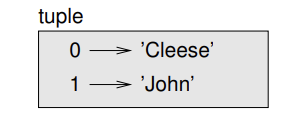
\includegraphics[width=0.5\textwidth]{./images/chapter_12_1.png}
        \caption{Diagrama de estados.}
        \label{fig:12_1}
        \end{figure}
        
\begin{figure}[h]
        \centering
        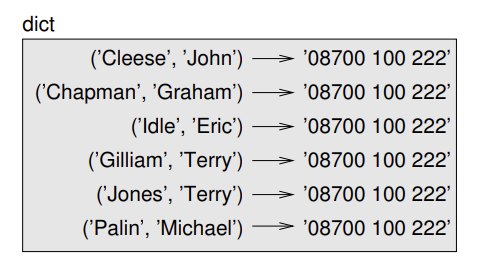
\includegraphics[width=0.5\textwidth]{./images/chapter_12_2.png}
        \caption{Diagrama de estados.}
        \label{fig:12_2}
        \end{figure}

\section{Secuencias de secuencias}

Me he centrado en listas de tuplas, pero casi todos los ejemplos de este capítulo también funcionan con listas de listas, tuplas de tuplas y tuplas de listas. Para evitar enumerar las posibles combinaciones, a veces es más fácil hablar de secuencias de secuencias.

En muchos contextos, los diferentes tipos de secuencias (cadenas, listas y tuplas) pueden usarse indistintamente. Entonces, ¿cómo elegir una sobre las otras?

Para empezar por lo obvio, las cadenas son más limitadas que otras secuencias porque los elementos tienen que ser caracteres. También son inmutables. Si necesitas la capacidad de cambiar los caracteres en una cadena (en lugar de crear una nueva cadena), podrías usar una lista de caracteres.

Las listas son más comunes que las tuplas, principalmente porque son mutables. Pero hay algunos casos donde podrías preferir tuplas:

1. En algunos contextos, como una sentencia \texttt{return}, es sintácticamente más simple crear una tupla que una lista.

2. Si quieres usar una secuencia como clave de diccionario, debes usar un tipo inmutable como una tupla o una cadena.

3. Si estás pasando una secuencia como argumento a una función, usar tuplas reduce el potencial de comportamientos inesperados debido a aliasing.

Como las tuplas son inmutables, no proporcionan métodos como \texttt{sort} y \texttt{reverse}, que modifican listas existentes. Pero Python proporciona la función incorporada \texttt{sorted}, que toma cualquier secuencia y devuelve una nueva lista con los mismos elementos en orden ordenado, y \texttt{reversed}, que toma una secuencia y devuelve un iterador que recorre la lista en orden inverso.

\section{Depuración}

Las listas, diccionarios y tuplas son ejemplos de estructuras de datos; en este capítulo estamos empezando a ver estructuras de datos compuestas, como listas de tuplas, o diccionarios que contienen tuplas como claves y listas como valores. Las estructuras de datos compuestas son útiles, pero son propensas a lo que llamo errores de forma; es decir, errores causados cuando una estructura de datos tiene el tipo, tamaño o estructura incorrectos. Por ejemplo, si esperas una lista con un entero y te doy un entero simple (no en una lista), no funcionará.

Para ayudar a depurar este tipo de errores, he escrito un módulo llamado \texttt{structshape} que proporciona una función, también llamada \texttt{structshape}, que toma cualquier tipo de estructura de datos como argumento y devuelve una cadena que resume su forma. Puedes descargarlo desde \url{https://thinkpython.com/code/structshape.py}

Aquí está el resultado para una lista simple:

\begin{lstlisting}[language=Python]
>>> from structshape import structshape
>>> t = [1, 2, 3]
>>> structshape(t)
'list of 3 int'
\end{lstlisting}

Un programa más elegante podría escribir "list of 3 ints", pero era más fácil no lidiar con plurales. Aquí hay una lista de listas:

\begin{lstlisting}[language=Python]
>>> t2 = [[1,2], [3,4], [5,6]]
>>> structshape(t2)
'list of 3 list of 2 int'
\end{lstlisting}

Si los elementos de la lista no son del mismo tipo, \texttt{structshape} los agrupa, en orden, por tipo:

\begin{lstlisting}[language=Python]
>>> t3 = [1, 2, 3, 4.0, '5', '6', [7], [8], 9]
>>> structshape(t3)
'list of (3 int, float, 2 str, 2 list of int, int)'
\end{lstlisting}

Aquí hay una lista de tuplas:

\begin{lstlisting}[language=Python]
>>> s = 'abc'
>>> lt = list(zip(t, s))
>>> structshape(lt)
'list of 3 tuple of (int, str)'
\end{lstlisting}

Y aquí hay un diccionario con 3 elementos que mapean enteros a cadenas:

\begin{lstlisting}[language=Python]
>>> d = dict(lt)
>>> structshape(d)
'dict of 3 int->str'
\end{lstlisting}

Si tienes problemas para mantener el seguimiento de tus estructuras de datos, \texttt{structshape} puede ayudarte.

\section{Glosario}

\begin{description}
\item[tupla:] Una secuencia inmutable de elementos.

\item[asignación de tuplas:] Una asignación con una secuencia en el lado derecho y una tupla de variables en el izquierdo. El lado derecho se evalúa y luego sus elementos se asignan a las variables de la izquierda.

\item[recolección:] Una operación que recoge múltiples argumentos en una tupla.

\item[dispersión:] Una operación que hace que una secuencia se comporte como múltiples argumentos.

\item[objeto zip:] El resultado de llamar a la función incorporada \texttt{zip}; un objeto que itera a través de una secuencia de tuplas.

\item[iterador:] Un objeto que puede iterar a través de una secuencia, pero que no proporciona operadores y métodos de listas.

\item[estructura de datos:] Una colección de valores relacionados, a menudo organizados en listas, diccionarios, tuplas, etc.

\item[error de forma:] Un error causado porque un valor tiene la forma incorrecta; es decir, el tipo o tamaño incorrecto.
\end{description}

\section{Ejercicios}

\textbf{Ejercicio 12.1.} Escribe una función llamada \texttt{most\_frequent} que tome una cadena e imprima las letras en orden decreciente de frecuencia. Encuentra muestras de texto en varios idiomas diferentes y observa cómo varía la frecuencia de las letras entre idiomas. Compara tus resultados con las tablas en \url{http://en.wikipedia.org/wiki/Letter_frequencies}. Solución: \url{https://thinkpython.com/code/most_frequent.py}.

\textbf{Ejercicio 12.2.} ¡Más anagramas!

1. Escribe un programa que lea una lista de palabras de un archivo (ver Sección 9.1) e imprima todos los conjuntos de palabras que son anagramas. Aquí hay un ejemplo de cómo podría verse la salida:

\begin{lstlisting}[language=Python]
['deltas', 'desalt', 'lasted', 'salted', 'slated', 'staled']
['retainers', 'ternaries']
['generating', 'greatening']
['resmelts', 'smelters', 'termless']
\end{lstlisting}

Pista: podrías construir un diccionario que mapee desde una colección de letras a una lista de palabras que se pueden escribir con esas letras. La pregunta es, ¿cómo puedes representar la colección de letras de una manera que se pueda usar como clave?

2. Modifica el programa anterior para que imprima la lista más larga de anagramas primero, seguida de la segunda más larga, y así sucesivamente.

3. En Scrabble, un "bingo" es cuando juegas las siete fichas de tu soporte, junto con una letra en el tablero, para formar una palabra de ocho letras. ¿Qué colección de 8 letras forma la mayor cantidad de bingos posibles? Solución: \url{https://thinkpython.com/code/anagram_sets.py}.

\textbf{Ejercicio 12.3.} Dos palabras forman un "par de metátesis" si puedes transformar una en la otra intercambiando dos letras; por ejemplo, "converse" y "conserve". Escribe un programa que encuentre todos los pares de metátesis en el diccionario. Pista: no pruebes todos los pares de palabras, y no pruebes todos los intercambios posibles. Solución: \url{https://thinkpython.com/code/metathesis.py}. Crédito: Este ejercicio está inspirado en un ejemplo en \url{http://puzzlers.org}.

\textbf{Ejercicio 12.4.} Aquí hay otro Puzzler de Car Talk (\url{http://www.cartalk.com/content/puzzlers}):

¿Cuál es la palabra más larga en inglés que sigue siendo una palabra válida en inglés a medida que eliminas sus letras una a una? Ahora, las letras se pueden eliminar de cualquier extremo o del medio, pero no puedes reorganizar ninguna de las letras. Cada vez que eliminas una letra, terminas con otra palabra en inglés. Si haces eso, eventualmente terminarás con una letra, y esa también será una palabra en inglés, una que se encuentre en el diccionario. Quiero saber cuál es la palabra más larga y cuántas letras tiene. Voy a darte un pequeño ejemplo modesto: Sprite. ¿Ok? Comienzas con sprite, quitas una letra, una del interior de la palabra, quitas la r, y nos queda spite, luego quitamos la e del final, nos queda spit, quitamos la s, nos queda pit, it, e I.

Escribe un programa para encontrar todas las palabras que se pueden reducir de esta manera y luego encuentra la más larga.

Este ejercicio es un poco más desafiante que la mayoría, así que aquí hay algunas sugerencias:

1. Podrías escribir una función que tome una palabra y calcule una lista de todas las palabras que se pueden formar eliminando una letra. Estas son las "hijas" de la palabra.

2. Recursivamente, una palabra es reducible si cualquiera de sus hijas es reducible. Como caso base, puedes considerar la cadena vacía reducible.

3. La lista de palabras que proporcioné, \texttt{words.txt}, no contiene palabras de una sola letra. Así que podrías agregar "I", "a" y la cadena vacía.

4. Para mejorar el rendimiento de tu programa, podrías memorizar las palabras que se sabe que son reducibles.

Solución: \url{https://thinkpython.com/code/reducible.py}.